% Options for packages loaded elsewhere
\PassOptionsToPackage{unicode}{hyperref}
\PassOptionsToPackage{hyphens}{url}
%
\documentclass[
]{book}
\usepackage{amsmath,amssymb}
\usepackage{lmodern}
\usepackage{ifxetex,ifluatex}
\ifnum 0\ifxetex 1\fi\ifluatex 1\fi=0 % if pdftex
  \usepackage[T1]{fontenc}
  \usepackage[utf8]{inputenc}
  \usepackage{textcomp} % provide euro and other symbols
\else % if luatex or xetex
  \usepackage{unicode-math}
  \defaultfontfeatures{Scale=MatchLowercase}
  \defaultfontfeatures[\rmfamily]{Ligatures=TeX,Scale=1}
\fi
% Use upquote if available, for straight quotes in verbatim environments
\IfFileExists{upquote.sty}{\usepackage{upquote}}{}
\IfFileExists{microtype.sty}{% use microtype if available
  \usepackage[]{microtype}
  \UseMicrotypeSet[protrusion]{basicmath} % disable protrusion for tt fonts
}{}
\makeatletter
\@ifundefined{KOMAClassName}{% if non-KOMA class
  \IfFileExists{parskip.sty}{%
    \usepackage{parskip}
  }{% else
    \setlength{\parindent}{0pt}
    \setlength{\parskip}{6pt plus 2pt minus 1pt}}
}{% if KOMA class
  \KOMAoptions{parskip=half}}
\makeatother
\usepackage{xcolor}
\IfFileExists{xurl.sty}{\usepackage{xurl}}{} % add URL line breaks if available
\IfFileExists{bookmark.sty}{\usepackage{bookmark}}{\usepackage{hyperref}}
\hypersetup{
  pdftitle={I am Bilingual - Python and R},
  pdfauthor={Priyanga Dilini Talagala   Thiyanga S. Talagala},
  hidelinks,
  pdfcreator={LaTeX via pandoc}}
\urlstyle{same} % disable monospaced font for URLs
\usepackage{color}
\usepackage{fancyvrb}
\newcommand{\VerbBar}{|}
\newcommand{\VERB}{\Verb[commandchars=\\\{\}]}
\DefineVerbatimEnvironment{Highlighting}{Verbatim}{commandchars=\\\{\}}
% Add ',fontsize=\small' for more characters per line
\usepackage{framed}
\definecolor{shadecolor}{RGB}{248,248,248}
\newenvironment{Shaded}{\begin{snugshade}}{\end{snugshade}}
\newcommand{\AlertTok}[1]{\textcolor[rgb]{0.94,0.16,0.16}{#1}}
\newcommand{\AnnotationTok}[1]{\textcolor[rgb]{0.56,0.35,0.01}{\textbf{\textit{#1}}}}
\newcommand{\AttributeTok}[1]{\textcolor[rgb]{0.77,0.63,0.00}{#1}}
\newcommand{\BaseNTok}[1]{\textcolor[rgb]{0.00,0.00,0.81}{#1}}
\newcommand{\BuiltInTok}[1]{#1}
\newcommand{\CharTok}[1]{\textcolor[rgb]{0.31,0.60,0.02}{#1}}
\newcommand{\CommentTok}[1]{\textcolor[rgb]{0.56,0.35,0.01}{\textit{#1}}}
\newcommand{\CommentVarTok}[1]{\textcolor[rgb]{0.56,0.35,0.01}{\textbf{\textit{#1}}}}
\newcommand{\ConstantTok}[1]{\textcolor[rgb]{0.00,0.00,0.00}{#1}}
\newcommand{\ControlFlowTok}[1]{\textcolor[rgb]{0.13,0.29,0.53}{\textbf{#1}}}
\newcommand{\DataTypeTok}[1]{\textcolor[rgb]{0.13,0.29,0.53}{#1}}
\newcommand{\DecValTok}[1]{\textcolor[rgb]{0.00,0.00,0.81}{#1}}
\newcommand{\DocumentationTok}[1]{\textcolor[rgb]{0.56,0.35,0.01}{\textbf{\textit{#1}}}}
\newcommand{\ErrorTok}[1]{\textcolor[rgb]{0.64,0.00,0.00}{\textbf{#1}}}
\newcommand{\ExtensionTok}[1]{#1}
\newcommand{\FloatTok}[1]{\textcolor[rgb]{0.00,0.00,0.81}{#1}}
\newcommand{\FunctionTok}[1]{\textcolor[rgb]{0.00,0.00,0.00}{#1}}
\newcommand{\ImportTok}[1]{#1}
\newcommand{\InformationTok}[1]{\textcolor[rgb]{0.56,0.35,0.01}{\textbf{\textit{#1}}}}
\newcommand{\KeywordTok}[1]{\textcolor[rgb]{0.13,0.29,0.53}{\textbf{#1}}}
\newcommand{\NormalTok}[1]{#1}
\newcommand{\OperatorTok}[1]{\textcolor[rgb]{0.81,0.36,0.00}{\textbf{#1}}}
\newcommand{\OtherTok}[1]{\textcolor[rgb]{0.56,0.35,0.01}{#1}}
\newcommand{\PreprocessorTok}[1]{\textcolor[rgb]{0.56,0.35,0.01}{\textit{#1}}}
\newcommand{\RegionMarkerTok}[1]{#1}
\newcommand{\SpecialCharTok}[1]{\textcolor[rgb]{0.00,0.00,0.00}{#1}}
\newcommand{\SpecialStringTok}[1]{\textcolor[rgb]{0.31,0.60,0.02}{#1}}
\newcommand{\StringTok}[1]{\textcolor[rgb]{0.31,0.60,0.02}{#1}}
\newcommand{\VariableTok}[1]{\textcolor[rgb]{0.00,0.00,0.00}{#1}}
\newcommand{\VerbatimStringTok}[1]{\textcolor[rgb]{0.31,0.60,0.02}{#1}}
\newcommand{\WarningTok}[1]{\textcolor[rgb]{0.56,0.35,0.01}{\textbf{\textit{#1}}}}
\usepackage{longtable,booktabs,array}
\usepackage{calc} % for calculating minipage widths
% Correct order of tables after \paragraph or \subparagraph
\usepackage{etoolbox}
\makeatletter
\patchcmd\longtable{\par}{\if@noskipsec\mbox{}\fi\par}{}{}
\makeatother
% Allow footnotes in longtable head/foot
\IfFileExists{footnotehyper.sty}{\usepackage{footnotehyper}}{\usepackage{footnote}}
\makesavenoteenv{longtable}
\usepackage{graphicx}
\makeatletter
\def\maxwidth{\ifdim\Gin@nat@width>\linewidth\linewidth\else\Gin@nat@width\fi}
\def\maxheight{\ifdim\Gin@nat@height>\textheight\textheight\else\Gin@nat@height\fi}
\makeatother
% Scale images if necessary, so that they will not overflow the page
% margins by default, and it is still possible to overwrite the defaults
% using explicit options in \includegraphics[width, height, ...]{}
\setkeys{Gin}{width=\maxwidth,height=\maxheight,keepaspectratio}
% Set default figure placement to htbp
\makeatletter
\def\fps@figure{htbp}
\makeatother
\setlength{\emergencystretch}{3em} % prevent overfull lines
\providecommand{\tightlist}{%
  \setlength{\itemsep}{0pt}\setlength{\parskip}{0pt}}
\setcounter{secnumdepth}{5}
\usepackage{booktabs}
\usepackage{amsthm}
\makeatletter
\def\thm@space@setup{%
  \thm@preskip=8pt plus 2pt minus 4pt
  \thm@postskip=\thm@preskip
}
\makeatother
\ifluatex
  \usepackage{selnolig}  % disable illegal ligatures
\fi
\usepackage[]{natbib}
\bibliographystyle{apalike}

\title{I am Bilingual - Python and R}
\author{Priyanga Dilini Talagala Thiyanga S. Talagala}
\date{2021-10-20}

\begin{document}
\maketitle

{
\setcounter{tocdepth}{1}
\tableofcontents
}
\hypertarget{preface}{%
\chapter*{Preface}\label{preface}}
\addcontentsline{toc}{chapter}{Preface}

WIP!!

\textbf{This book is still in progress in various draft forms.}

\hypertarget{intro}{%
\chapter{Introduction to R and Python}\label{intro}}

R Vs Python: What's the Difference? \url{https://www.guru99.com/r-vs-python.html}

\hypertarget{about-r-and-python}{%
\section{About R and Python}\label{about-r-and-python}}

\hypertarget{r}{%
\subsection{R}\label{r}}

R is an object oriented, open source programming \textbf{language} and \textbf{environment} for statistical computing and graphics. R is not a statistics system but an environment within which statistical techniques are implemented. Further, R gains more capabilities via packages, its fundamental shareable units that bundle together R functions, code, data, documentation, and tests etc. \citep{Rcoreteam2020}.

\hypertarget{python}{%
\subsection{Python}\label{python}}

Python is an object-oriented, interpreted, and interactive programming language. The motto of Python language is ``Batteries included'' as the functionality of the language can be performed via its comprehensive standard in built Libraries \citep{wikipython}.

\hypertarget{history-of-r-and-python}{%
\section{History of R and Python}\label{history-of-r-and-python}}

\hypertarget{r-1}{%
\subsection{R}\label{r-1}}

R is an implementation of the S programming language which was created by John Chambers in 1976. In 1991, an alternative implementation of the basic S language was developed by Ross Ihaka and Robert Gentleman, University of Auckland, New Zealand. It was published in 1993 \citep{wikiR}.

\hypertarget{python-1}{%
\subsection{Python}\label{python-1}}

In 1989, Guido van Rossum at Centrum Wiskunde \& Informatica (CWI) in the Netherlands started the implementation of Python as a successor to ABC programming language. Python 2.0 was released in 2000. Python 3.0, a major revision of the language that is not completely backward-compatible was released in 2008 \citep{wikipython} . Today many developers create libraries strictly for the use with Python 3.

\hypertarget{story-behind-their-names}{%
\section{Story behind their names}\label{story-behind-their-names}}

\hypertarget{r-2}{%
\subsection{R}\label{r-2}}

R was introduced by \textbf{R}oss Ihaka and \textbf{R}obert Gentleman and it was named after the first names of the two authors. The name of the ``S'' language also had some influence on the selection of its name and it was selected partly as a play on the name of S \citep{wikiR}.

\hypertarget{python-2}{%
\subsection{Python}\label{python-2}}

Python was named after a famous \href{https://en.wikipedia.org/wiki/Monty_Python\%27s_Flying_Circus}{TV show `Monty Python's Flying Circus'}. Guido van Rossum, the creater of Python was a big fan of the TV show. He wanted to name his invention with a short, unique and slightly mysterious name and chose Python as a working title for his ongoing project.

\hypertarget{logo}{%
\section{Logo}\label{logo}}

\begin{figure}

{\centering 
\includegraphics[width=0.3\linewidth]{fig/C1_Rlogo} 

}

\caption{Retrieved from: https://www.r-project.org/logo/}\label{fig:unnamed-chunk-1}
\end{figure}

\begin{figure}

{\centering 
\includegraphics[width=0.6\linewidth]{fig/C1_Pythonlogo} 

}

\caption{Retrieved from: https://www.python.org/community/logos/}\label{fig:unnamed-chunk-2}
\end{figure}

\hypertarget{worldwide-google-trends}{%
\section{Worldwide Google Trends}\label{worldwide-google-trends}}

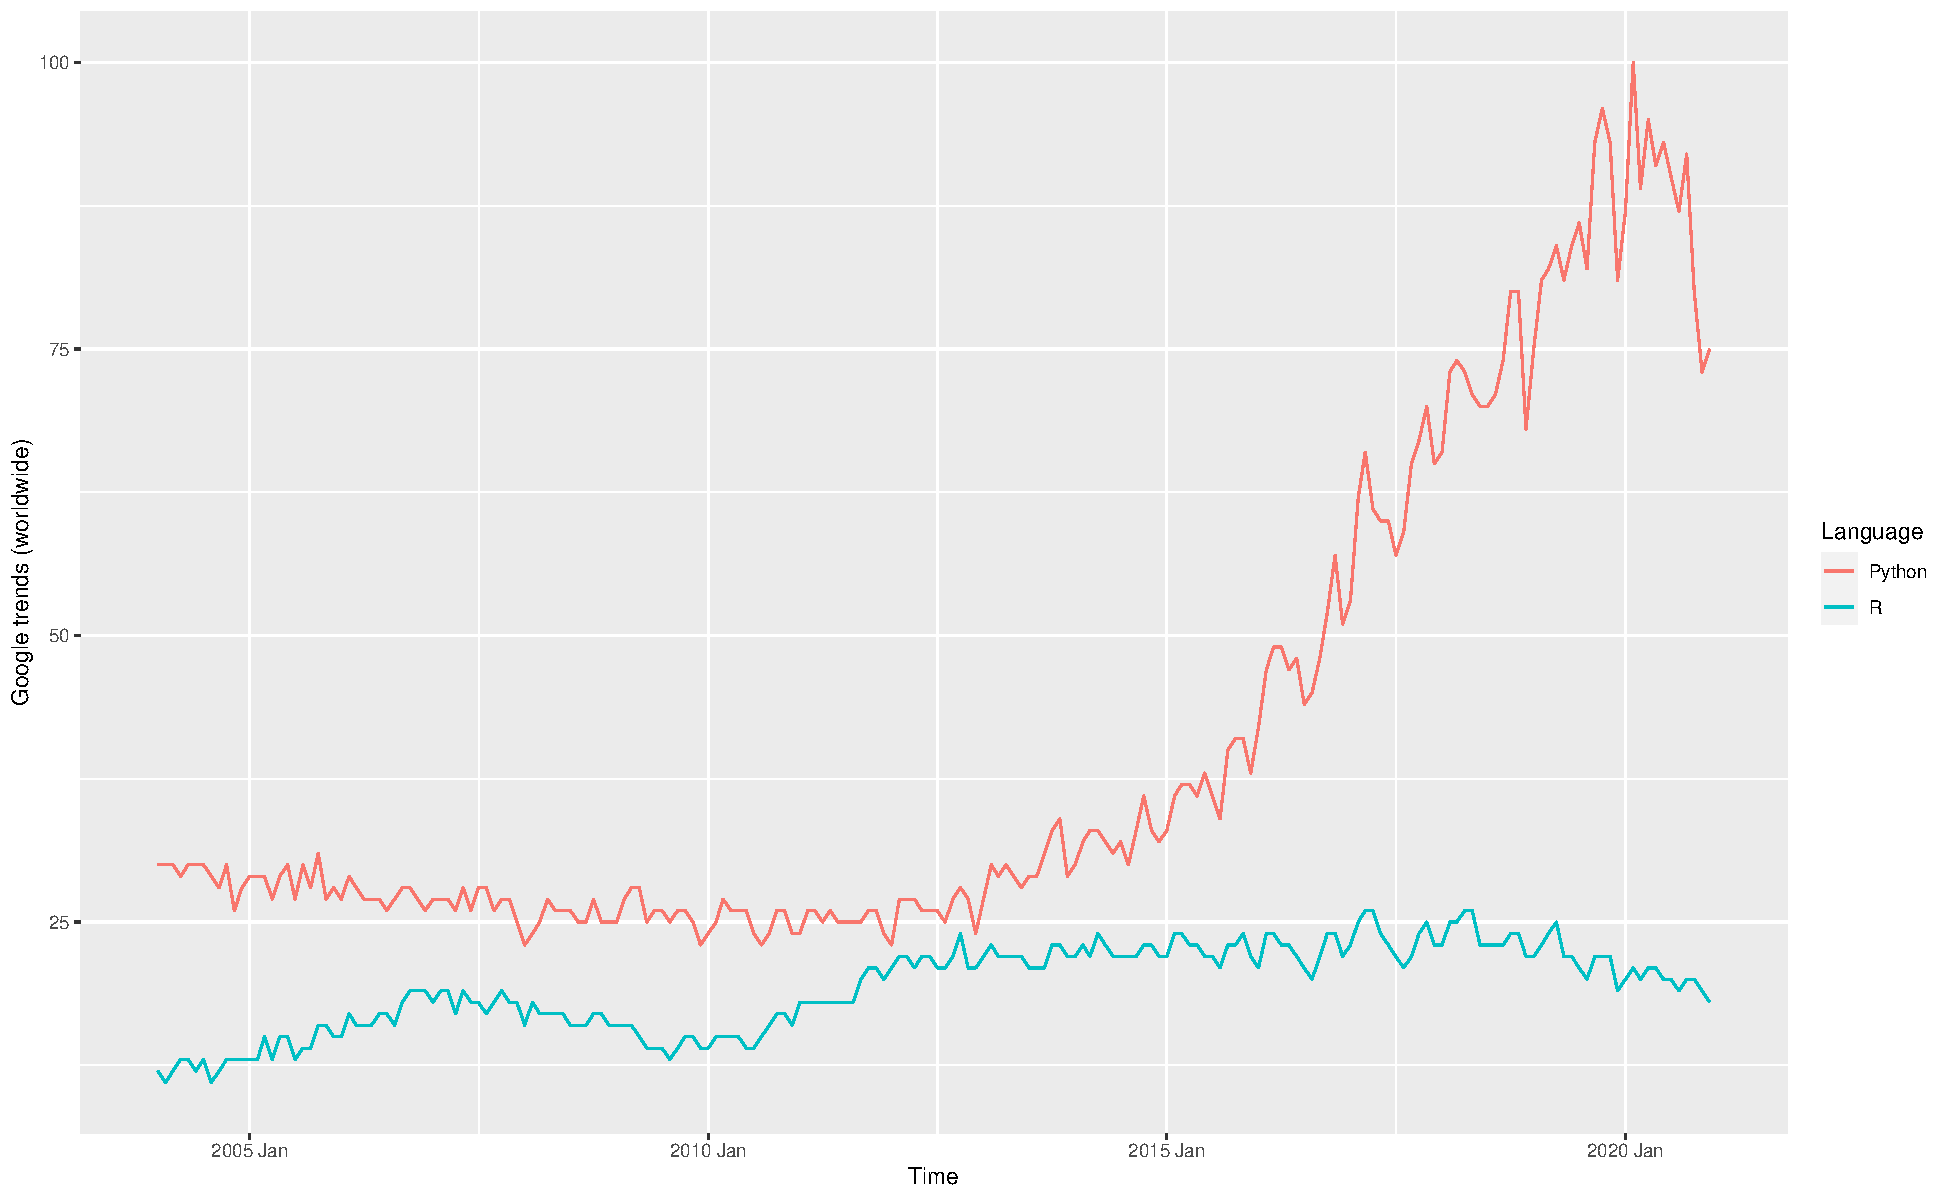
\includegraphics{IamBilingual_files/figure-latex/googletrends-1.pdf}

\hypertarget{installation}{%
\section{Installation}\label{installation}}

\hypertarget{r-3}{%
\subsection{R}\label{r-3}}

You can download it for free from the following websites:
- R (\url{https://cran.r-project.org/})

\textbf{Install Rstudio IDE}

RStudio is an integrated development environment for R, a programming language for statistical computing and graphics. It is available in two formats: RStudio Desktop is a regular desktop application while RStudio Server runs on a remote server and allows accessing RStudio using a web browser.

\begin{itemize}
\tightlist
\item
  RStudio (\url{https://www.rstudio.com/products/rstudio/download/\#download}).
\end{itemize}

\hypertarget{python-3}{%
\subsection{Python}\label{python-3}}

Ref: \url{https://www.w3schools.com/python/python_getstarted.asp}

Many PCs and Macs will have python already installed.

To check if you have python installed on a Windows PC, search in the start bar for Python or run the following on the Command Line (cmd.exe):

\texttt{C:\textbackslash{}Users\textbackslash{}Your\ Name\textgreater{}python\ -\/-version}

To check if you have python installed on a Linux or Mac, then on linux open the command line or on Mac open the Terminal and type:

\texttt{python\ -\/-version}

If you find that you do not have python installed on your computer, then you can download it for free from the following website: \url{https://www.python.org/}

\textbf{Install PyCharm IDE}

PyCharm is a cross-platform IDE that provides consistent experience on the Windows, macOS, and Linux operating systems.

PyCharm is available in three editions: Professional, Community, and Edu. The Community and Edu editions are open-source projects and they are free, but they have fewer features. PyCharm Edu provides courses and helps you learn programming with Python. The Professional edition is commercial, and provides an outstanding set of tools and features. For details, see the editions comparison matrix.

\hypertarget{install-and-load-libraries}{%
\section{Install and Load Libraries}\label{install-and-load-libraries}}

\hypertarget{r-4}{%
\subsection{R}\label{r-4}}

R Packages: A Beginner's Guide \url{https://www.datacamp.com/community/tutorials/r-packages-guide?utm_source=adwords_ppc\&utm_campaignid=1655852085\&utm_adgroupid=61045434222\&utm_device=c\&utm_keyword=\%2Bload\%20\%2Bpackage\%20\%2Br\&utm_matchtype=b\&utm_network=g\&utm_adpostion=\&utm_creative=469789579329\&utm_targetid=aud-522010995285:kwd-589281898774\&utm_loc_interest_ms=9071445\&utm_loc_physical_ms=1009919\&gclid=Cj0KCQjwyZmEBhCpARIsALIzmnKGh4ZVHa4OxhLq0JUzpoBMMRhQvCGEmvscFuLZ5CI3V3JPsQ2v9P8aAhwpEALw_wcB}

An \textbf{R package} is a way to organize your own work and share it with others. Typically, a package contains code, documentation for the package and the functions inside, some tests to check everything works as it should, and data sets.

Three of the most popular repositories for R packages are: CRAN, Bioconductor and Github.

\hypertarget{installing-packages-from-cran}{%
\subsubsection{Installing Packages From CRAN}\label{installing-packages-from-cran}}

\texttt{install.packages("package\_name")}

Example

\texttt{install.packages("tidyverse")}

After running this, some messages will be diplayed on the console. They will depend on what operating system you are using, the dependencies, and if the package was successfully installed.

To install more than a package at the same time, we can use a character vector

\texttt{install.packages(c("vioplot",\ "MASS"))}

\textbf{The function \texttt{install.packages} will download the source code from on the CRAN mirrors and install the package (and any dependencies) locally on your computer.}

You have to install a package only once.

\hypertarget{load-packages}{%
\subsubsection{Load Packages}\label{load-packages}}

After a package is installed, you are ready to use its functionalities.

If you just need a sporadic use of a few functions or data inside a package you can access them with the notation

\texttt{packagename::functionname()}.

If you will make a more intensive use of the package, then maybe is worth to load it into memory. The simplest way to do this is with the \texttt{library()} command.

Please note that the input of install.packages() is a character vector and requires the name to be in quotes, while library() accepts either character or name and makes it possible for you to write the name of the package without quotes.

Once you have the package installed, you can load the library into your R session for use. Any of the functions that are specific to that package will be available for you to use by simply calling the function as you would for any of the base functions. Note that quotations are not required here.

\texttt{library(tidyverse)}

\hypertarget{python-4}{%
\subsection{Python}\label{python-4}}

Use `import module' or `from module import'? \url{https://stackoverflow.com/questions/710551/use-import-module-or-from-module-import}

\textbf{Method 1:} \texttt{import\ module}

\textbf{Method 2:} \texttt{from\ module\ import\ foo}

The difference between \texttt{import\ module} and \texttt{from\ module\ import\ foo} is subjective. User can select one method and be consitent in the use of it.

\begin{longtable}[]{@{}
  >{\raggedright\arraybackslash}p{(\columnwidth - 2\tabcolsep) * \real{0.42}}
  >{\raggedright\arraybackslash}p{(\columnwidth - 2\tabcolsep) * \real{0.58}}@{}}
\toprule
\texttt{import\ module} & \texttt{from\ module\ import\ foo} \\
\midrule
\endhead
\textbf{Pros} & \textbf{Pros} \\
- Less Maintanence of the import statements & - Less typying to use \texttt{foo} function \\
- Don't need to add any aditional imports to start using another item from the same module & - More control over whcih items of the module can be accessed \\
\textbf{Cons} & \textbf{Cons} \\
- Typing \texttt{module.foo} in the code be tedious (dull, boring ) & to use new items from the module the user have to update the \texttt{import} statement \\
\bottomrule
\end{longtable}

\begin{itemize}
\tightlist
\item
  It can be minimized by using \texttt{import\ module\ as\ mo}, then typing \texttt{mo.foo} \textbar{} You loose context about \texttt{foo}. For example it is less clear \texttt{ceil()} does, compared to \texttt{math.ceil()}
\end{itemize}

\textbf{Don't use}

\begin{itemize}
\item
  \texttt{from\ modle\ import\ *}

  \begin{itemize}
  \tightlist
  \item
    Because it clutters or fills with untidy collection of things in the namespace
  \end{itemize}
\item
  \texttt{import\ *}

  \begin{itemize}
  \item
    For any reasonable large set of code, if you \texttt{import\ *} you will likely be cementing it into the module, unable to be removed.
  \item
    This is because now it is difficullt to identiify what items used in the code are coming from \texttt{module}.
  \end{itemize}
\end{itemize}

\hypertarget{ranked15python-packages}{%
\section{Ranked:15Python packages}\label{ranked15python-packages}}

for Data Science

\url{http://blog.thedataincubator.com/wp-content/uploads/2017/04/Ranked-15-Python-Packages-for-Data-Science.pdf}

\hypertarget{variables-expressions-and-statements}{%
\chapter{Variables, expressions, and statements}\label{variables-expressions-and-statements}}

\hypertarget{basic-exmaple}{%
\section{Basic Exmaple}\label{basic-exmaple}}

This is a test code

\hypertarget{r-code}{%
\subsection{R code}\label{r-code}}

\begin{Shaded}
\begin{Highlighting}[]
\CommentTok{\# This is an R code}
\NormalTok{x }\OtherTok{\textless{}{-}} \DecValTok{1}
\NormalTok{y }\OtherTok{\textless{}{-}} \DecValTok{3}
\FunctionTok{print}\NormalTok{(x}\SpecialCharTok{+}\NormalTok{y)}
\end{Highlighting}
\end{Shaded}

\begin{verbatim}
## [1] 4
\end{verbatim}

\hypertarget{python-code}{%
\subsection{Python Code}\label{python-code}}

The `python' engine in knitr requires the \texttt{reticulate} package.

\begin{Shaded}
\begin{Highlighting}[]
\FunctionTok{library}\NormalTok{(reticulate)}
\end{Highlighting}
\end{Shaded}

\begin{Shaded}
\begin{Highlighting}[]
\CommentTok{\# This is a Python code}
\NormalTok{x }\OperatorTok{=} \DecValTok{1}
\NormalTok{y }\OperatorTok{=} \DecValTok{3}
\BuiltInTok{print}\NormalTok{(x}\OperatorTok{+}\NormalTok{y)}
\end{Highlighting}
\end{Shaded}

\begin{verbatim}
## 4
\end{verbatim}

\hypertarget{conditional-execution}{%
\chapter{Conditional execution}\label{conditional-execution}}

WIP

\hypertarget{functions}{%
\chapter{Functions}\label{functions}}

WIP

\hypertarget{iteration}{%
\chapter{Iteration}\label{iteration}}

WIP

\hypertarget{tidy-workflow}{%
\chapter{Tidy workflow}\label{tidy-workflow}}

WIP

Moving from R to Python: The Libraries You Need to Know \url{https://www.kdnuggets.com/2017/02/moving-r-python-libraries.html}

\hypertarget{import}{%
\chapter{Import}\label{import}}

WIP

\hypertarget{tidy}{%
\chapter{Tidy}\label{tidy}}

WIP

\hypertarget{transform}{%
\chapter{Transform}\label{transform}}

WIP

\hypertarget{data-visualization}{%
\chapter{Data Visualization}\label{data-visualization}}

\hypertarget{data}{%
\section{Data}\label{data}}

The Palmer penguins dataset was introduced by Allison Horst, Alison Hill, and Kristen Gorman provide a great dataset for data exploration and visualization, as an alternative to iris. It was first introduced as an R package. The released version of palmerpenguins can be instaalled from CRAN with:

\textbf{R Installation}
\texttt{install.packages("palmerpenguins")}

Using \href{https://pypi.org/project/palmerpenguins/}{\texttt{palmerpenguins} python package} you can easily load the Palmer penguins into your python environment.

\textbf{Python Installation}
\texttt{pip\ install\ palmerpenguins}

The palmerpenguins package contains two datasets : \texttt{penguins} and \texttt{penguins\_raw}. \texttt{penguins} is a simplified version of the \texttt{penguins\_raw} data.

\hypertarget{r-5}{%
\section{R}\label{r-5}}

\textbf{Load data}

\begin{Shaded}
\begin{Highlighting}[]
\CommentTok{\# Load Palmer Archipelago (Antarctica) Penguin Data}
\FunctionTok{library}\NormalTok{(palmerpenguins)}
\CommentTok{\# Return the first part of the dataset}
\FunctionTok{head}\NormalTok{(penguins)}
\end{Highlighting}
\end{Shaded}

\begin{verbatim}
## # A tibble: 6 x 8
##   species island bill_length_mm bill_depth_mm flipper_length_~ body_mass_g sex  
##   <fct>   <fct>           <dbl>         <dbl>            <int>       <int> <fct>
## 1 Adelie  Torge~           39.1          18.7              181        3750 male 
## 2 Adelie  Torge~           39.5          17.4              186        3800 fema~
## 3 Adelie  Torge~           40.3          18                195        3250 fema~
## 4 Adelie  Torge~           NA            NA                 NA          NA <NA> 
## 5 Adelie  Torge~           36.7          19.3              193        3450 fema~
## 6 Adelie  Torge~           39.3          20.6              190        3650 male 
## # ... with 1 more variable: year <int>
\end{verbatim}

\begin{Shaded}
\begin{Highlighting}[]
\CommentTok{\# Retrieve column names}
\FunctionTok{colnames}\NormalTok{(penguins)}
\end{Highlighting}
\end{Shaded}

\begin{verbatim}
## [1] "species"           "island"            "bill_length_mm"   
## [4] "bill_depth_mm"     "flipper_length_mm" "body_mass_g"      
## [7] "sex"               "year"
\end{verbatim}

\hypertarget{base-r-package}{%
\subsection{\texorpdfstring{\texttt{base} R package}{base R package}}\label{base-r-package}}

\begin{Shaded}
\begin{Highlighting}[]
\CommentTok{\# Define color for each of the 3 penguine species}
\NormalTok{colors }\OtherTok{\textless{}{-}} \FunctionTok{c}\NormalTok{(}\StringTok{"\#00AFBB"}\NormalTok{, }\StringTok{"\#E7B800"}\NormalTok{, }\StringTok{"\#FC4E07"}\NormalTok{)}
\NormalTok{colors }\OtherTok{\textless{}{-}}\NormalTok{ colors[}\FunctionTok{as.numeric}\NormalTok{(penguins}\SpecialCharTok{$}\NormalTok{species)]}

\CommentTok{\# Define shapes}
\NormalTok{shapes }\OtherTok{=} \FunctionTok{c}\NormalTok{(}\DecValTok{16}\NormalTok{, }\DecValTok{17}\NormalTok{, }\DecValTok{18}\NormalTok{) }
\NormalTok{shapes }\OtherTok{\textless{}{-}}\NormalTok{ shapes[}\FunctionTok{as.numeric}\NormalTok{(penguins}\SpecialCharTok{$}\NormalTok{species)]}

\FunctionTok{plot}\NormalTok{(}\AttributeTok{x =}\NormalTok{ penguins}\SpecialCharTok{$}\NormalTok{flipper\_length\_mm,}
          \AttributeTok{y =}\NormalTok{ penguins}\SpecialCharTok{$}\NormalTok{body\_mass\_g,}
          \AttributeTok{col =}\NormalTok{ colors,}
          \AttributeTok{pch =}\NormalTok{ shapes,}
          \AttributeTok{xlab =} \StringTok{"Flipper Length"}\NormalTok{,}
          \AttributeTok{ylab =} \StringTok{"Body Mass"}\NormalTok{ )}
\end{Highlighting}
\end{Shaded}

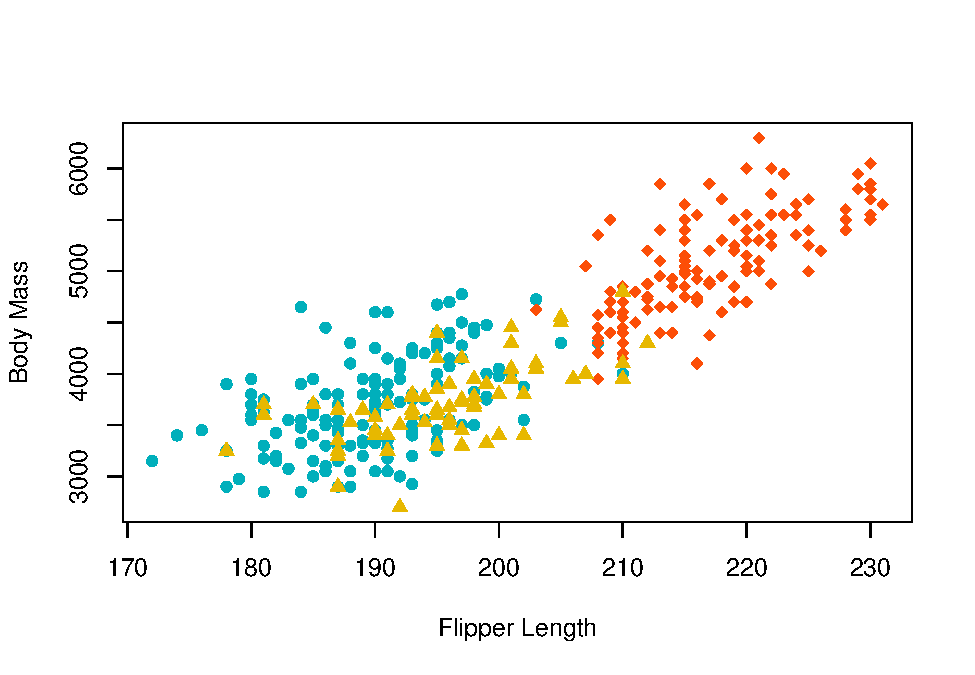
\includegraphics{IamBilingual_files/figure-latex/unnamed-chunk-6-1.pdf}

\hypertarget{gggplot2-package}{%
\subsection{\texorpdfstring{\texttt{gggplot2} Package}{gggplot2 Package}}\label{gggplot2-package}}

\texttt{ggplot2} is an R package dedicated to data visualization which is based on The Grammar of Graphics \citep{wilkinson2012grammar}.

\begin{Shaded}
\begin{Highlighting}[]
\CommentTok{\#load ggplot2 package to make statistical graphics}
\FunctionTok{library}\NormalTok{(ggplot2)}
\NormalTok{p }\OtherTok{\textless{}{-}} \FunctionTok{ggplot}\NormalTok{(penguins) }\SpecialCharTok{+}
  \FunctionTok{geom\_point}\NormalTok{( }\FunctionTok{aes}\NormalTok{(}\AttributeTok{x =}\NormalTok{ flipper\_length\_mm,}
                  \AttributeTok{y =}\NormalTok{ body\_mass\_g,}
                  \AttributeTok{color =}\NormalTok{ species,}
                  \AttributeTok{shape =}\NormalTok{ species)) }\SpecialCharTok{+}
  \FunctionTok{xlab}\NormalTok{(}\StringTok{"Flipper Length"}\NormalTok{)}\SpecialCharTok{+}
  \FunctionTok{ylab}\NormalTok{(}\StringTok{"Body Mass"}\NormalTok{)}

\FunctionTok{print}\NormalTok{(p)}
\end{Highlighting}
\end{Shaded}

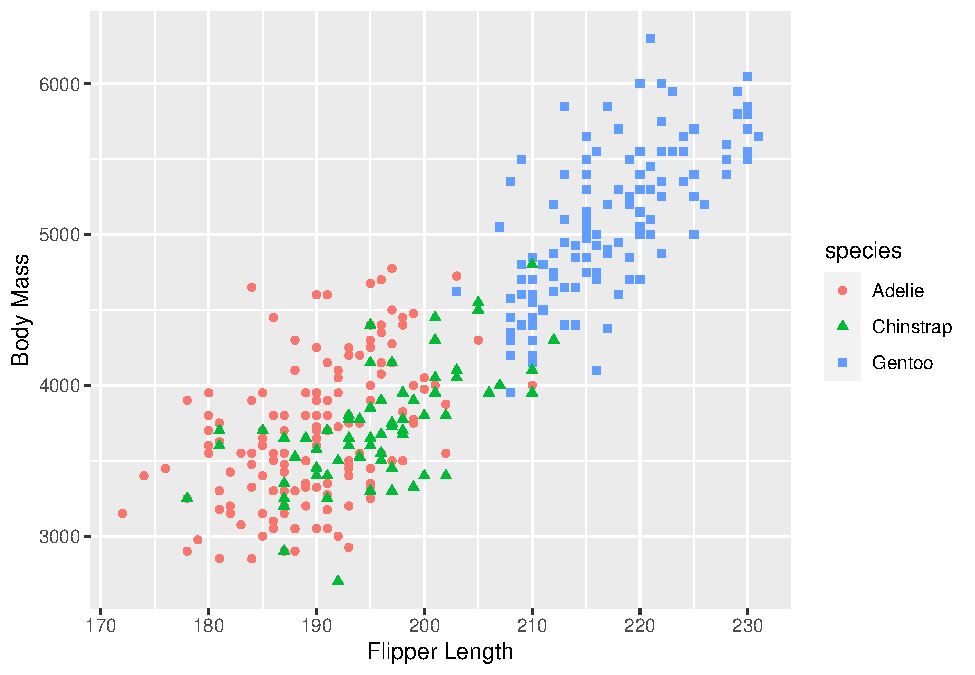
\includegraphics{IamBilingual_files/figure-latex/unnamed-chunk-7-1.pdf}

\hypertarget{plotly-r-package-for-interactive-data-visualization}{%
\subsection{\texorpdfstring{\texttt{plotly} R package for interactive data visualization}{plotly R package for interactive data visualization}}\label{plotly-r-package-for-interactive-data-visualization}}

Interactive visualization focuses on graphic representations of data that improve the way we interact with information

plotly is an R package for creating interactive web-based graphs via the open source JavaScript graphing library plotly.js.

\begin{Shaded}
\begin{Highlighting}[]
\FunctionTok{library}\NormalTok{(plotly)}
\NormalTok{p }\OtherTok{\textless{}{-}} \FunctionTok{ggplot}\NormalTok{(penguins) }\SpecialCharTok{+}
  \FunctionTok{geom\_point}\NormalTok{( }\FunctionTok{aes}\NormalTok{(}\AttributeTok{x =}\NormalTok{ flipper\_length\_mm,}
                  \AttributeTok{y =}\NormalTok{ body\_mass\_g,}
                  \AttributeTok{color =}\NormalTok{ species,}
                  \AttributeTok{shape =}\NormalTok{ species)) }\SpecialCharTok{+}
  \FunctionTok{xlab}\NormalTok{(}\StringTok{"Flipper Length"}\NormalTok{)}\SpecialCharTok{+}
  \FunctionTok{ylab}\NormalTok{(}\StringTok{"Body Mass"}\NormalTok{)}

\CommentTok{\# The function ggplotly converts a ggplot2::ggplot() object to a plotly object.}
\NormalTok{plotly}\SpecialCharTok{::}\FunctionTok{ggplotly}\NormalTok{(p)}
\end{Highlighting}
\end{Shaded}

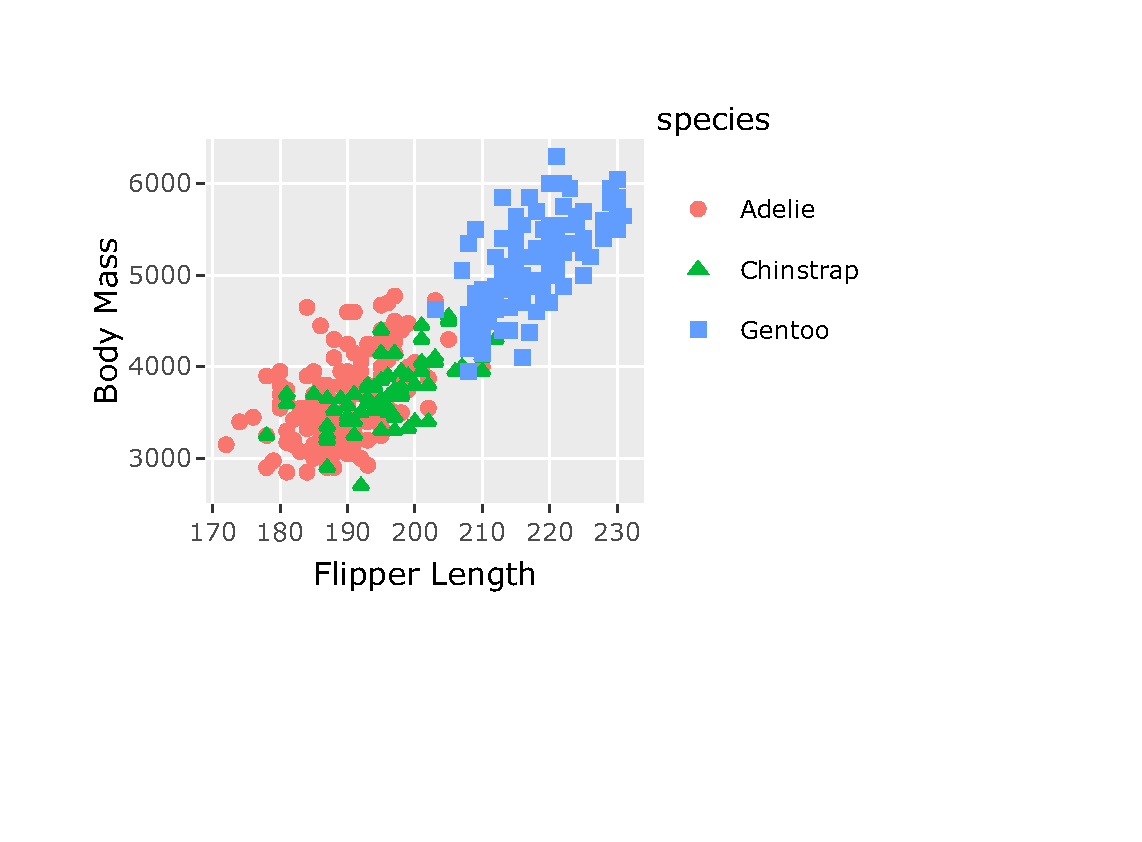
\includegraphics{IamBilingual_files/figure-latex/unnamed-chunk-8-1.pdf}

\textbf{Method 2}

\begin{Shaded}
\begin{Highlighting}[]
\FunctionTok{library}\NormalTok{(plotly)}
\NormalTok{fig }\OtherTok{\textless{}{-}} \FunctionTok{plot\_ly}\NormalTok{(penguins, }
               \AttributeTok{x =} \SpecialCharTok{\textasciitilde{}}\NormalTok{flipper\_length\_mm,}
               \AttributeTok{y =} \SpecialCharTok{\textasciitilde{}}\NormalTok{body\_mass\_g, }
               \AttributeTok{color =} \SpecialCharTok{\textasciitilde{}}\NormalTok{species,}
               \AttributeTok{symbol =} \SpecialCharTok{\textasciitilde{}}\NormalTok{species,}
               \AttributeTok{type =} \StringTok{"scatter"}\NormalTok{)}
\NormalTok{fig}
\end{Highlighting}
\end{Shaded}

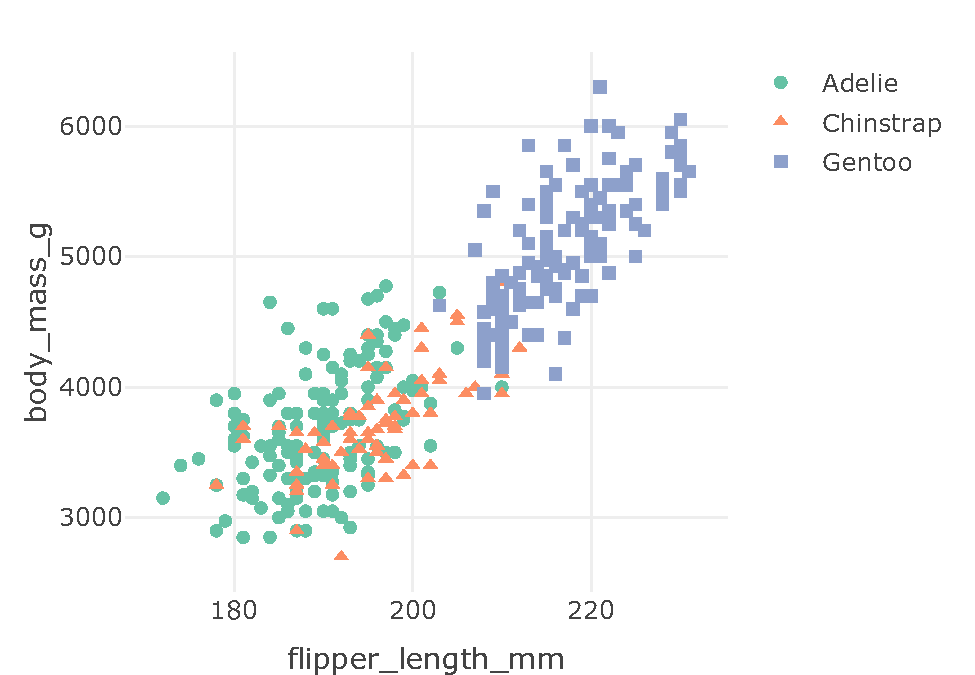
\includegraphics{IamBilingual_files/figure-latex/unnamed-chunk-9-1.pdf}

\hypertarget{python-5}{%
\section{Python}\label{python-5}}

\textbf{Load data}

\begin{Shaded}
\begin{Highlighting}[]
\CommentTok{\#load functions in palmerpenguins package}
\ImportTok{from}\NormalTok{ palmerpenguins }\ImportTok{import}\NormalTok{ load\_penguins}
\NormalTok{penguins }\OperatorTok{=}\NormalTok{ load\_penguins()}
\CommentTok{\# Return the first part of the dataset}
\NormalTok{penguins.head()}
\CommentTok{\# Retrieve column names}
\BuiltInTok{list}\NormalTok{(penguins.columns)}
\end{Highlighting}
\end{Shaded}

\hypertarget{matplotlib-package}{%
\subsection{\texorpdfstring{\texttt{Matplotlib} package}{Matplotlib package}}\label{matplotlib-package}}

Matplotlib is mainly deployed for basic plotting. Visualization using Matplotlib generally consists of bars, pies, lines, scatter plots and so on.

\begin{Shaded}
\begin{Highlighting}[]
\CommentTok{\# Import matplotlib to make statistical graphics. }
\CommentTok{\# By convention, it is imported with the shorthand sns.}
\ImportTok{import}\NormalTok{ matplotlib.pyplot }\ImportTok{as}\NormalTok{ plt}

\NormalTok{colors }\OperatorTok{=}\NormalTok{ \{}\StringTok{\textquotesingle{}Adelie\textquotesingle{}}\NormalTok{:}\StringTok{\textquotesingle{}blue\textquotesingle{}}\NormalTok{, }\StringTok{\textquotesingle{}Gentoo\textquotesingle{}}\NormalTok{:}\StringTok{\textquotesingle{}orange\textquotesingle{}}\NormalTok{, }\StringTok{\textquotesingle{}Chinstrap\textquotesingle{}}\NormalTok{:}\StringTok{\textquotesingle{}green\textquotesingle{}}\NormalTok{\}}
\NormalTok{plt.scatter(penguins.flipper\_length\_mm,}
\NormalTok{penguins.body\_mass\_g, }
\NormalTok{c}\OperatorTok{=}\NormalTok{ penguins.species.}\BuiltInTok{apply}\NormalTok{(}\KeywordTok{lambda}\NormalTok{ x: colors[x]))}
\NormalTok{plt.xlabel(}\StringTok{\textquotesingle{}Flipper Length\textquotesingle{}}\NormalTok{)}
\NormalTok{plt.ylabel(}\StringTok{\textquotesingle{}Body Mass\textquotesingle{}}\NormalTok{)}
\end{Highlighting}
\end{Shaded}

\begin{center}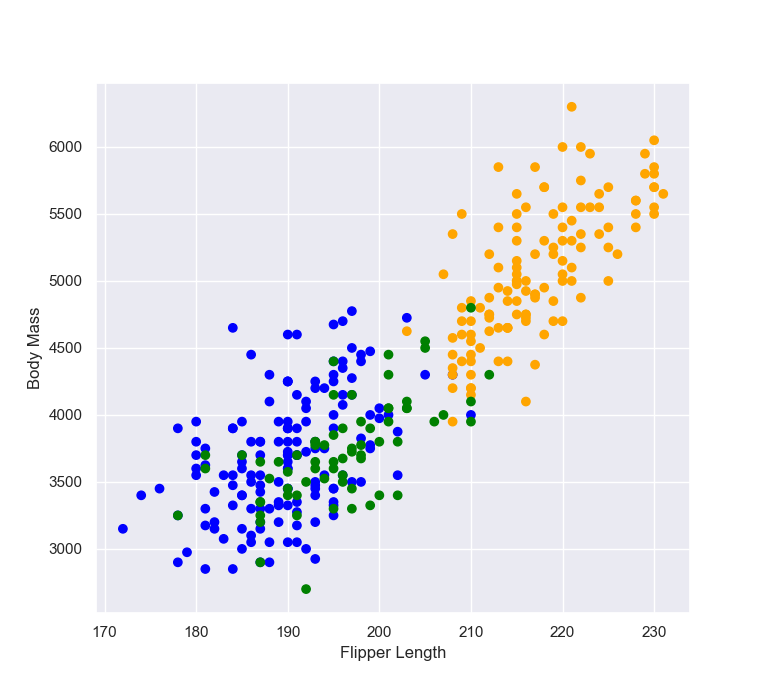
\includegraphics[width=0.9\linewidth]{fig/Viz_chap/1_matplot} \end{center}

\hypertarget{seaborn-package}{%
\subsection{\texorpdfstring{\texttt{seaborn} Package}{seaborn Package}}\label{seaborn-package}}

Seaborn is an easy-to-use high level statistical plotting library which provides a variety of visualization patterns. It uses fewer syntax and has easily interesting default themes.

It tries to provide a `grammar of graphics' style way to create plots but in a pythonic style without getting the exact syntax from ggplot as in plotnine.

\href{https://elitedatascience.com/python-seaborn-tutorial}{Introduction to Seaborn}

\begin{Shaded}
\begin{Highlighting}[]
\CommentTok{\# Import seaborn to make statistical graphics. }
\CommentTok{\# By convention, it is imported with the shorthand sns.}
\ImportTok{import}\NormalTok{ seaborn }\ImportTok{as}\NormalTok{ sns }
\CommentTok{\#load functions in palmerpenguins package}
\ImportTok{from}\NormalTok{ palmerpenguins }\ImportTok{import}\NormalTok{ load\_penguins}
\NormalTok{penguins }\OperatorTok{=}\NormalTok{ load\_penguins()}

\CommentTok{\# Apply the default theme}
\NormalTok{sns.set\_theme()}
\CommentTok{\# sns.set\_style(\textquotesingle{}whitegrid\textquotesingle{})}
\NormalTok{p }\OperatorTok{=}\NormalTok{ sns.relplot(x }\OperatorTok{=} \StringTok{\textquotesingle{}flipper\_length\_mm\textquotesingle{}}\NormalTok{,}
\NormalTok{            y }\OperatorTok{=}\StringTok{\textquotesingle{}body\_mass\_g\textquotesingle{}}\NormalTok{,}
\NormalTok{            hue }\OperatorTok{=} \StringTok{\textquotesingle{}species\textquotesingle{}}\NormalTok{,}
\NormalTok{            style }\OperatorTok{=} \StringTok{\textquotesingle{}species\textquotesingle{}}\NormalTok{,}
\NormalTok{            data }\OperatorTok{=}\NormalTok{ penguins)}
\NormalTok{p.set\_xlabels(}\StringTok{\textquotesingle{}Flipper Length\textquotesingle{}}\NormalTok{)}
\NormalTok{p.set\_ylabels(}\StringTok{\textquotesingle{}Body Mass\textquotesingle{}}\NormalTok{)   }
\end{Highlighting}
\end{Shaded}

\begin{center}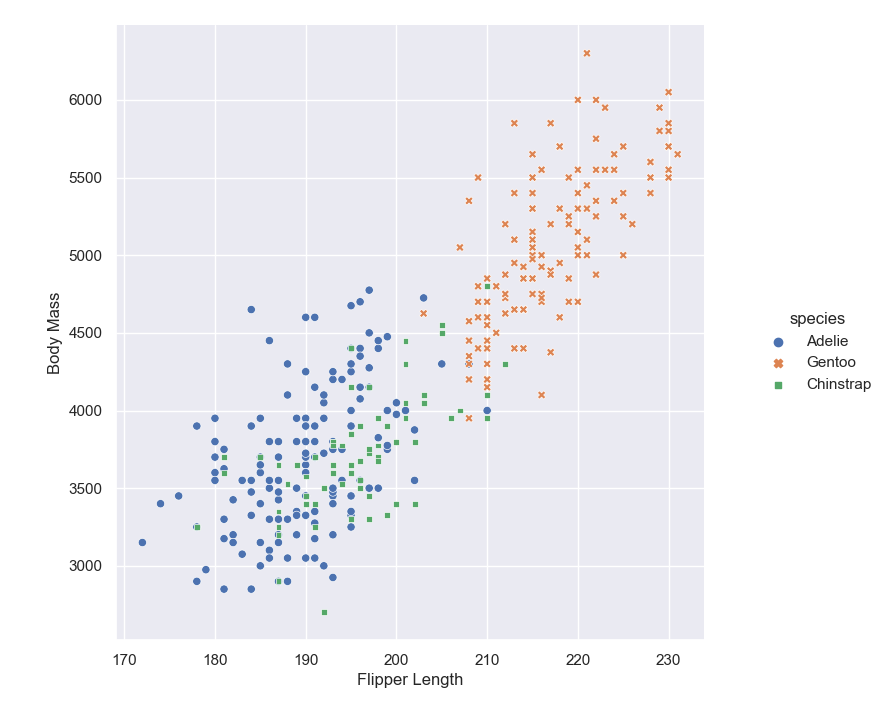
\includegraphics[width=0.9\linewidth]{fig/Viz_chap/2_seaborn} \end{center}

The function \texttt{relplot()} is named that way because it is designed to visualize many different statistical relationships. The \texttt{relplot()} function has a convenient kind parameter that lets you easily switch to this alternate representation:
\texttt{scatterplot()} with \texttt{kind="scatter"}; the default and \texttt{lineplot()} with \texttt{kind="line"}.

\hypertarget{plotnine-package}{%
\subsection{\texorpdfstring{\texttt{plotnine} package}{plotnine package}}\label{plotnine-package}}

\url{https://pypi.org/project/plotnine/}

plotnine is an implementation of a grammar of graphics in Python, it is based on ggplot2. The grammar allows users to compose plots by explicitly mapping data to the visual objects that make up the plot.

Plotting with a grammar is powerful, it makes custom (and otherwise complex) plots are easy to think about and then create, while the simple plots remain simple.

\textbf{NOTE: R vs Python Syntax}

\textbf{Unlike in R, now all the variables must be enclosed by single quotes}

\begin{Shaded}
\begin{Highlighting}[]
\ImportTok{from}\NormalTok{ plotnine }\ImportTok{import} \OperatorTok{*}
\CommentTok{\# unlike in R, now all the variables must be enclosed by single quotes}
\NormalTok{(ggplot(penguins) }\OperatorTok{+}
\NormalTok{  geom\_point(aes(x }\OperatorTok{=} \StringTok{\textquotesingle{}flipper\_length\_mm\textquotesingle{}}\NormalTok{,}
\NormalTok{                  y }\OperatorTok{=} \StringTok{\textquotesingle{}body\_mass\_g\textquotesingle{}}\NormalTok{,}
\NormalTok{                  color }\OperatorTok{=} \StringTok{\textquotesingle{}species\textquotesingle{}}\NormalTok{,}
\NormalTok{                  shape }\OperatorTok{=} \StringTok{\textquotesingle{}species\textquotesingle{}}\NormalTok{)) }\OperatorTok{+}
\NormalTok{  xlab(}\StringTok{"Flipper Length"}\NormalTok{)}\OperatorTok{+}
\NormalTok{  ylab(}\StringTok{"Body Mass"}\NormalTok{))}
\end{Highlighting}
\end{Shaded}

\begin{center}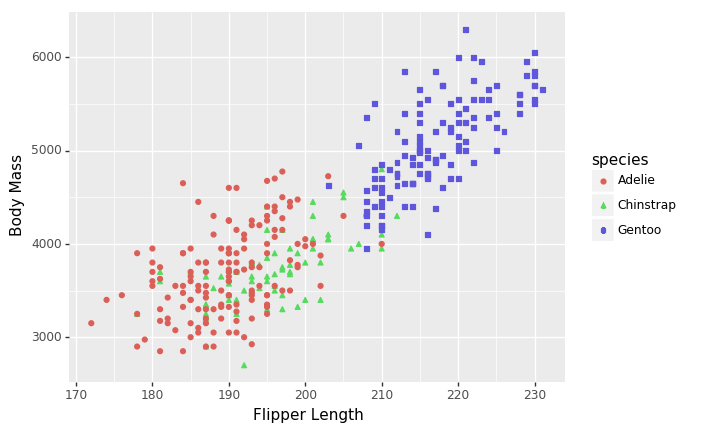
\includegraphics[width=0.9\linewidth]{fig/Viz_chap/3_plotnine} \end{center}

\hypertarget{plotly-python-library-for-interactive-data-visualization}{%
\subsection{\texorpdfstring{\texttt{plotly} Python library for interactive data visualization}{plotly Python library for interactive data visualization}}\label{plotly-python-library-for-interactive-data-visualization}}

The \texttt{plotly.express} (Plotly Express or PX) module contains functions that can create entire figures at once. It is usually imported as \texttt{px}. Plotly Express is a built-in part of the \texttt{plotly} library.

\begin{Shaded}
\begin{Highlighting}[]
\ImportTok{import}\NormalTok{ plotly.express }\ImportTok{as}\NormalTok{ px}

\NormalTok{fig }\OperatorTok{=}\NormalTok{ px.scatter(penguins,}
\NormalTok{                 x}\OperatorTok{=}\StringTok{"flipper\_length\_mm"}\NormalTok{,}
\NormalTok{                 y}\OperatorTok{=}\StringTok{"body\_mass\_g"}\NormalTok{,}
\NormalTok{                 color}\OperatorTok{=} \StringTok{"species"}\NormalTok{,}
\NormalTok{                 symbol}\OperatorTok{=} \StringTok{"species"}\NormalTok{,}
\NormalTok{                 labels}\OperatorTok{=}\BuiltInTok{dict}\NormalTok{(flipper\_length\_mm}\OperatorTok{=}\StringTok{"Flipper Length"}\NormalTok{,}
\NormalTok{                             body\_mass\_g}\OperatorTok{=}\StringTok{"Body Mass"}\NormalTok{))}
\NormalTok{fig.show()}
\end{Highlighting}
\end{Shaded}

\hypertarget{model}{%
\chapter{Model}\label{model}}

WIP

\hypertarget{communicate}{%
\chapter{Communicate}\label{communicate}}

WIP

\hypertarget{advanced-r-and-python}{%
\chapter{Advanced R and Python}\label{advanced-r-and-python}}

WIP

\hypertarget{time-series-forecasting}{%
\section{Time Series Forecasting}\label{time-series-forecasting}}

\begin{longtable}[]{@{}
  >{\raggedright\arraybackslash}p{(\columnwidth - 2\tabcolsep) * \real{0.50}}
  >{\raggedright\arraybackslash}p{(\columnwidth - 2\tabcolsep) * \real{0.50}}@{}}
\toprule
R & Python \\
\midrule
\endhead
\href{https://cran.r-project.org/web/packages/fable/index.html}{fable}-Forecasting Models for Tidy Time Series & \href{https://www.statsmodels.org/devel/user-guide.html\#time-series-analysis}{statsmodels}- Statistics based models \\
\href{https://cran.r-project.org/web/packages/forecast/index.html}{forecast}- Forecasting Functions for Time Series and Linear Models & \href{https://www.sktime.org/en/latest/}{sktime}- A unified framework for machine learning with time series \\
\(\text{}\) & \href{https://ts.gluon.ai/}{GluonTS}- Deep learning-based models. \\
\bottomrule
\end{longtable}

\hypertarget{jupyter-notebooks}{%
\chapter{Jupyter Notebooks}\label{jupyter-notebooks}}

\begin{itemize}
\tightlist
\item
  The \href{https://jupyter.org/}{Jupyter Notebook} is an open-source web application that allows the user to create and share documents that contain live code, equations, visualizations, and narrative text.
\item
  \href{https://jupyter.org/}{JupyterLab} is an advanced version of Jupyter Notebook interface. It brings the classic notebooks, text editor, terminal, and directory viewer all under one roof. However, both operate in a similar fashion.
\end{itemize}

\hypertarget{how-to-install-jupyter-environment}{%
\section{How to install Jupyter environment?}\label{how-to-install-jupyter-environment}}

First, open a new command prompt (Windows) or terminal (Mac/Linux) on your workstation, and second, execute the following command:

\texttt{jupyter\ notebook}

If the above command fails, first, you need to install python on your workstation. There are two popular methods to install Python on your workstation.

\begin{itemize}
\tightlist
\item
  Installing Python using Anaconda Distribution
\item
  Installing Raw Python
\end{itemize}

\href{https://blog.quantinsti.com/jupyter-notebook-tutorial-installation-components-magic-commands/?source=google\&medium=cpc\&campaign=dsa_other_topnations\&gclid=CjwKCAjw_L6LBhBbEiwA4c46ui3I3LExNsT-8hio3gGLkVRXewJwHZO3EijzgRAkh29lx7uCg8P4hxoCGuAQAvD_BwE}{Click on this link}. It will guide you to install python.

\begin{itemize}
\tightlist
\item
  After installing python using one of the above methods, then we need to installing Jupyter Notebook using either Anaconda or pip.
\end{itemize}

\hypertarget{how-to-run-or-open-jupyter-notebooks}{%
\section{How to run or open Jupyter Notebooks?}\label{how-to-run-or-open-jupyter-notebooks}}

\begin{itemize}
\item
  After you have installed the Jupyter Notebook on your computer, you are ready to run the notebook server.
\item
  Keep the terminal open as it is. It will then open the default web browser with the URL mentioned in the command prompt or terminal.
\item
  When the notebook opens in your browser, you will see the Notebook Homepage
\end{itemize}

\hypertarget{shutdown-the-jupyter-notebook-local-server}{%
\section{Shutdown the Jupyter Notebook Local Server}\label{shutdown-the-jupyter-notebook-local-server}}

\begin{itemize}
\item
  You can also close your terminal by typing the command \texttt{exit} and hitting \texttt{Enter}.
\item
  You can also shutdown a Jupyter Notebook session by clicking in the Terminal window and clicking \texttt{Ctrl+c}. You will be asked to confirm that you want to Shutdown this notebook server (y/{[}n{]})?. Type y and hit Enter to confirm. Then, you can close the Terminal by typing the command exit and hitting Enter.
\end{itemize}

\hypertarget{working-with-jupyter-notebook}{%
\chapter{Working with jupyter notebook}\label{working-with-jupyter-notebook}}

\begin{enumerate}
\def\labelenumi{\arabic{enumi}.}
\tightlist
\item
  open temrinal
\item
  Type \texttt{jupyter\ notebook}
\item
  Go to --\textgreater{} new --\textgreater{} folder (or select and exiting folder from the files list)
\item
  Then creat jupyter notebook
  new--\textgreater{} Python 3
\end{enumerate}

\hypertarget{working-with-pycharm}{%
\chapter{Working with pycharm}\label{working-with-pycharm}}

\begin{enumerate}
\def\labelenumi{\arabic{enumi}.}
\tightlist
\item
  First install pycharm
\item
  Open pycharm
\item
  Create a project (select a location)
\item
  Open terminal
\item
  Type \texttt{jupyter\ notebook}
\item
  Create jupyter notebook
\item
  Quit notebook
\end{enumerate}

\hypertarget{install-packages}{%
\section{install packages}\label{install-packages}}

\texttt{python\ -m\ pip\ install\ \textless{}package\textgreater{}}

must read what toavoide: \url{https://jakevdp.github.io/blog/2017/12/05/installing-python-packages-from-jupyter/}

\hypertarget{install-python-package-using-jupyter-notebook}{%
\section{Install Python package using Jupyter Notebook}\label{install-python-package-using-jupyter-notebook}}

\begin{itemize}
\tightlist
\item
  \url{https://www.geeksforgeeks.org/install-python-package-using-jupyter-notebook/}
\end{itemize}

\texttt{import\ sys\ !\{sys.executable\}\ -m\ pip\ install\ {[}package\_name{]}}

  \bibliography{book.bib}

\end{document}
